
\section{Background}
We present the framework of GANs starting with the original paper by Ian Goodfellow \cite{goodfellow2014generative} then describe more recent advances in a chronological order, as depicted in Figure \ref{fig:background-timeline}. 
% Summarize a few notable approaches/papers tackling the same problem. The selection should cover different possible techniques that can be (have been) used for the same task with success. Also, it is good to mention other recognition/synthesis tasks that use the same deep learning technique as yours. (1-2 pages)

\begin{figure}
\centering
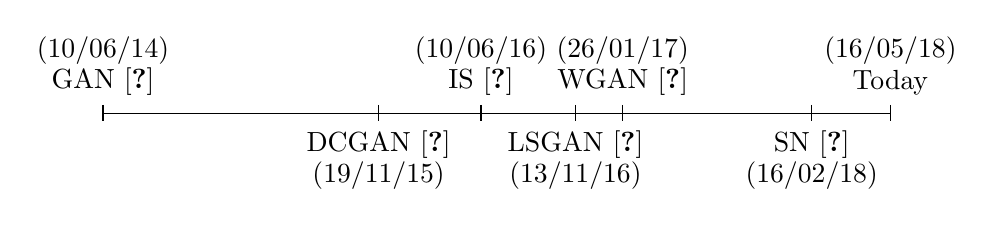
\begin{tikzpicture}
\draw (0,0) -- (10,0);

% draw vertical lines
\foreach \x in {0,3.5,4.8,6.0,6.6,9.0,10.0}
\draw (\x cm,3pt) -- (\x cm,-3pt);

% draw nodes
% 1 yr is roughly 2.5 units
\draw (0,0) node[above=3pt] {GAN \cite{goodfellow2014generative}};
\draw (0,0) node[above=14pt] {(10/06/14)};

\draw (3.5,0) node[below=3pt] {DCGAN \cite{DBLP:journals/corr/RadfordMC15}};
\draw (3.5,0) node[below=14pt] {(19/11/15)};

\draw (4.8,0) node[above=3pt] {IS \cite{salimans2016improved}};
\draw (4.8,0) node[above=14pt] {(10/06/16)};

\draw (6,0) node[below=3pt] {LSGAN \cite{mao2017least}};
\draw (6,0) node[below=14pt] {(13/11/16)};

\draw (6.6,0) node[above=3pt] {WGAN \cite{arjovsky2017wasserstein}};
\draw (6.6,0) node[above=14pt] {(26/01/17)};

\draw (9.0,0) node[below=3pt] {SN \cite{salimans2016improved}};
\draw (9.0,0) node[below=14pt] {(16/02/18)};

\draw (10.0,0) node[above=3pt] {Today};
\draw (10.0,0) node[above=14pt] {(16/05/18)};

\end{tikzpicture}
\caption{Major contributions in the field of Generative Adversarial Networks.}
\label{fig:background-timeline}
\end{figure}


% 2014 jun 10: GAN
% 2015 nov 19: DCGAN
% 2016 jun 10: IS
% 2016 nov 13: LSGAN
% 2017 jan 26: WGAN 
% 2018 feb 16: SN  
% 2018 may 16: Today 

\subsection{Generative Adversarial Networks} 
Generative Adversarial Networks (GANs) were first introduced in \cite{goodfellow2014generative}. They are a class of generative models trained in a adversarial manner by opposing two networks: a generative network $G$ that learns the data distribution and a discriminative network $D$ that tries and estimates the probability that a given sample came from the real training data rather than a generation from $G$. 
 
The objective for $G$ is to maximize the probability of $D$ making a mistake, and the objective for $D$ is to minimize that same probability. This framework corresponds to a minimax two-player game. In the space of arbitrary functions $G$ and $D$, a unique equilibrium solution exists, with $G$ recovering the real data distribution and $D$ equal to 0.5 everywhere, meaning it's unable to distinguish the real images from the ones generated by $G$. Since $G$ and $D$ are (de-)convolutional networks, both can be trained using available backpropagation techniques.

To learn the distribution $p_g$ over the real data $\bm{x}$, $G$ starts from sampling input variables $\bm{z}$ from a distribution of our choice $p_z(\bm{z})$, then maps the input variables $\bm{z}$ to space $G(\bm{z}; \theta_g)$ that should, after training, resemble the training data space. The discriminator, $D$, maps images to a boolean $D(\bm{x}; \theta_d)$ indicating whether images are from training data or generated from $G$. The orignal minimax objective for GANs is defined as:
\begin{equation}
\label{eq_gan}
\min_G \max_D V_{\text{\tiny GAN}}(D, G) = \mathbb{E}_{\bm{x} \sim p_{\text{data}}(\bm{x})}[\log D(\bm{x})] + \mathbb{E}_{\bm{z} \sim p_{\bm{z}}(\bm{z})}[\log (1 - D(G(\bm{z})))] .
\end{equation}

\subsection{Deep Convolutional Generative Adversarial Networks}
Building upon Goodfellow's work \cite{goodfellow2014generative}, Radford et al. apply the GAN framework to computer vision, bridging the gap between the success of Convolutional Neural Networks (CNNs)for supervised learning and GANs for unsupervised learning \cite{DBLP:journals/corr/RadfordMC15}. Training on various image datasets, authors show that the adversarial pair learns a hierarchy of features in both the generator and discriminator. 

\subsection{Inception Score}
The Inception Score (IS) is first presented in \cite{salimans2016improved}. This work (originating from OpenAI, whose team includes author of the original GAN paper Ian Goodfellow) presents a variety of new architectural features and training procedures meant to improve the training of GANs. Amongst other things, authors make the observation that GANs lack an objective function, which making it difficult to compare the performance of different models. In the context of image generation, an intuitive performance metric can be obtained by human annotators assessing the quality of the generated images. However, this method isn't as scalable as one would wish for obvious reasons. The inception score is proposed as an alternative, and is shown to correlate well with human evaluation. 

We describe the method briefly. By applying the Inception model \cite{inceptionv2} to all generated images, we get the conditional label distribution $p(y|\bm{x})$. Images that contain meaningful objects should have a conditional label distribution $p(y|\bm{x})$ with low entropy. Moreover, we expect the model to generate varied images, so the marginal $\int p(y|\bm{x} = G(z))dz$ should have high entropy. By combining these two requirements, the proposed metric becomes: 

%$\exp( \mathbb{E}_{\bm{x}} \text{KL} (p(y|\bm{x})||p(y)))$, where results are exponentiated so that values are easier to compare.
% In \cite{Barrat2018IS} the Inception score is defined  as:
\begin{equation}
\label{eq_IS}
\begin{split}
IS(G) = exp\big(\mathbb{E}_{\bm{x} \sim p_{\text{data}}(\bm{x})}D_{KL}(p(y|\bm{x})||p(y))\big).
\end{split}
\end{equation}

Here $D_{KL}$ is known as the Kullback Libler divergence and it measures how one probability distribution diverges from another by using a logarithmic difference:
\begin{eqnarray}
	D_{\mathrm {KL} }(P\|Q)=\int _{-\infty }^{\infty }p(x)\,\log {\frac {p(x)}{q(x)}}\,dx
\end{eqnarray}
 $p(y|\bm{x})$ is the conditional label distribution while $p(y)$ is the  marginalized label distribution, i.e. $p(y)=\int_{\bm{x}} (p(y|\bm{x})p_g(\bm{x}) d\bm{x}$. In order to calculate the score we replace $p(y)$ with the empirical marginal class distribution $\hat{p}(y) = \sum^N_{i=1} p(y|\bm{x}^i)$ and estimate the expectation using the basic Monte Carlo estimator yielding:

\begin{equation}
\label{eq_IS2}
\begin{split}
IS(G) = exp\big(\sum^N_{i=1}D_{KL}(p(y|\bm{x}^i)||\hat{p}(y))\big).
\end{split}
\end{equation}


\subsection{Least Squares Generative Adversarial Networks}
% Taken as is from LSGAN paper
Viewing the discriminator as a classifier, regular GANs adopt the sigmoid cross entropy loss function. As stated in Section \ref{sec:introduction}, when updating the generator, this loss function will cause the problem of vanishing gradients for the samples that are on the correct side of the decision boundary, but are still far from the real data. To remedy this problem, we propose the Least Squares Generative Adversarial Networks (LSGANs). Suppose we use the $a$-$b$ coding scheme for the discriminator, where $a$ and $b$ are the labels for fake data and real data,  respectively. Then the objective functions for LSGANs can be defined as follows:

\begin{equation}
\label{eq:lsgan}
\begin{split}
\min_D V_{\text{\tiny LSGAN}}(D) = &\frac{1}{2}\mathbb{E}_{\bm{x} \sim p_{\text{data}}(\bm{x})}\bigl[(D(\bm{x})-b)^2\bigr]+ \frac{1}{2}\mathbb{E}_{\bm{z} \sim p_{\bm{z}}(\bm{z})}\bigl[(D(G(\bm{z}))-a)^2\bigr] \\
\min_G V_{\text{\tiny LSGAN}}(G) = &\frac{1}{2}\mathbb{E}_{\bm{z} \sim p_{\bm{z}}(\bm{z})}\bigl[(D(G(\bm{z}))-c)^2\bigr],
\end{split}
\end{equation}


where $c$ denotes the value that $G$ wants $D$ to believe for fake data.

\subsubsection{Benefits of LSGANs}
The benefits of LSGANs can be derived from two aspects. First, unlike regular GANs, which cause almost no loss for samples that lie in a long way on the correct side of the decision boundary (Figure \ref{fig:boundary}(b)), LSGANs will penalize those samples even though they are correctly classified (Figure \ref{fig:boundary}(c)). When we update the generator, the parameters of the discriminator are fixed, i.e., the decision boundary is fixed. As a result, the penalization will make the generator to generate samples toward the decision boundary. On the other hand, the decision boundary should go across the manifold of real data for a successful GANs learning. Otherwise, the learning process will be saturated. Thus moving the generated samples toward the decision boundary leads to making them be closer to the manifold of real data. 

Second, penalizing the samples lying a long way to the decision boundary can generate more gradients when updating the generator, which in turn relieves the problem of vanishing gradients. This allows LSGANs to perform more stable during the learning process. This benefit can also be derived from another perspective: as shown in Figure \ref{fig:loss}, the least squares loss function is flat only at one point, while the sigmoid cross entropy loss function will saturate when $x$ is relatively large.

\subsection{WGAN}


\todo{Cite authors of WGAN saying ``Weight clipping is a clearly terrible way to enforce a Lipschitz constraint''}

Recommended clip limit is 0.01

\subsection{Spectral Normalization}



